
\section{问题重述}



\subsection{背景介绍}

随着2024年该校将教师课堂教学评价任务下放至各学院自行组织,尽管此举旨在提升效率,但也随之带来了评分标准异质性、量尺使用偏差以及内部评价过程可能存在的系统性偏差等一系列挑战。具体表现为学院间评分区间差异显著、得分分布特性不一,以及部分学院内部评分机制可能引入局部偏差,这些因素均可能影响教师教学质量评价的客观性与公平性。本文需分析:

教师课堂教学评价是高校职称评定体系的重要组成部分。
在高校教师职称评定过程中,课堂教学评分是衡量教师教学质量的重要依据。传统上,学校通常由教务处或教师发展中心聘请有资质的专家团队,对候选教师逐门课程的课堂表现进行多维度评分并加总总分,作为职称与评优决策参考。然而,评分专家组成、评价尺度及个人打分习惯的不同,可能导致一定程度的主观偏差。随着参评教师基数逐年增加,部分高校为提升评价效率、缓解管理压力,尝试将部分评价任务下放到各学院自评。此举在减轻负担的同时,也产生了评分标准不统一等新问题。
2023年,学校集中组织了两组专家分别对同一批教师进行了多指标评分。本文需分析:
\begin{enumerate}
    \item 两组专家对同批教师的评分结果之间是否存在统计学上的显著性差异?
    \item 哪一组专家评分结果在信度和一致性上更值得信赖?
\end{enumerate}


\subsection{问题提出}
\textbf\textit{{问题一}}
分析附件1中学校组织的两组专家对同一批教师的教学评价结果有无显著性差异,哪一组结果更可信?

\textbf{问题二} 
根据附件2中的数据,分析各个学院的打分特点与规律,给出一种合理的汇总方式,在此基础上建立数学模型,重新计算所有教师的教学评分,并对结果的合理性进行解释。

\begin{enumerate}
    \item 如何深入分析附件2中各学院的教学评分数据,识别并量化其在评分标准、打分范围和内部一致性等方面的特点与规律?
    \item 如何提出并建立一个合理的数学模型,以有效消除或减少因学院间差异带来的偏差,对所有教师的教学评分进行重新计算与校准?
    \item 如何对经过模型重新计算后的教师教学评分结果的公平性、有效性及合理性进行全面阐释?
\end{enumerate}






% \subsection{Background}

% Juneau, the capital city of Alaska, seamlessly combines 
% breathtaking natural beauty with a rich cultural heritage. 
% Nestled in the southeastern part of the state, this unique city 
% is accessible only by air or sea, giving it an island-like allure 
% despite being located on the mainland. Home to approximately 30,000 
% residents, Juneau welcomes over a million tourists annually—a number 
% that continues to grow each year. While tourism has significantly 
% boosted the city’s economy, it has also brought challenges, such 
% as receding glaciers, increasingly crowded streets, and rising 
% carbon emissions. To ensure its long-term prosperity, Juneau 
% must embrace a \textbf{sustainable tourism strategy} that balances growth 
% with the preservation of its natural and cultural treasures, which will be
% presented in the following sections.


% \subsection{Restatement and Analyses of the Problem}

% We need to complete the following tasks based on the given background
% and our collected data.

% \begin{itemize}
%     \item \textbf{Task 1: Develop a model to quantify the tourism industry in Juneau and analyse the model.}
%     \begin{itemize}
%         \item The model is required to qualitatively and quantitatively analyze the factors that affect the tourism industry in Juneau, including the economy, society, and environment. 
%         \item The model should be able to predict the number of tourists in the next few years and provide insights into the development of the tourism industry in Juneau.
%         \item A sensitivity anslysis should be conducted to evaluate the robustness of the model.
%     \end{itemize}
%     \item \textbf{Task 2: Test the model's adaptability and migration capability in Sitka, Alaska.}
%     \\Based on the model developed in Task 1, we need to adapt the model to the city of Sitka, Alaska, and test its adaptability and migration capability.
%     \item \textbf{Task 3: Propose a sustainable tourism strategy for Juneau.}
%     \\Based on the model developed in Task 1, we need to propose a sustainable tourism strategy for Juneau that balances economic growth with environmental and social sustainability.
% \end{itemize}

% It can be noted that task 1 serves as the foundation for Task 2 and Task 3, 
% while Task 2 provides a practical application of the model developed in Task 1. 
% Task 3 aims to address the challenges and opportunities identified in Task 1 and Task 2, 
% providing a comprehensive and sustainable solution for the tourism industry in Juneau.

% Questions can be asked to further clarify the problem:
% How to quantify the tourism industry in Juneau? Which factors should be 
% considered in the model and what methods should be used? After developing 
% the model, how can we adapt it to another city? What suggestions and 
% strategies can be proposed to promote the sustainable development of the
% tourism industry in Juneau?

% In summary, we should effectively build a model that can quantify the tourism
% industry in Juneau, adapt the model to another city, and propose a sustainable
% tourism strategy for Juneau.


% \subsection{Overview of Our Work}

% On the basis of the above analyses we carried out out work and the 
% working framework is shown below.

% \begin{figure}[H]
%     \centering
%     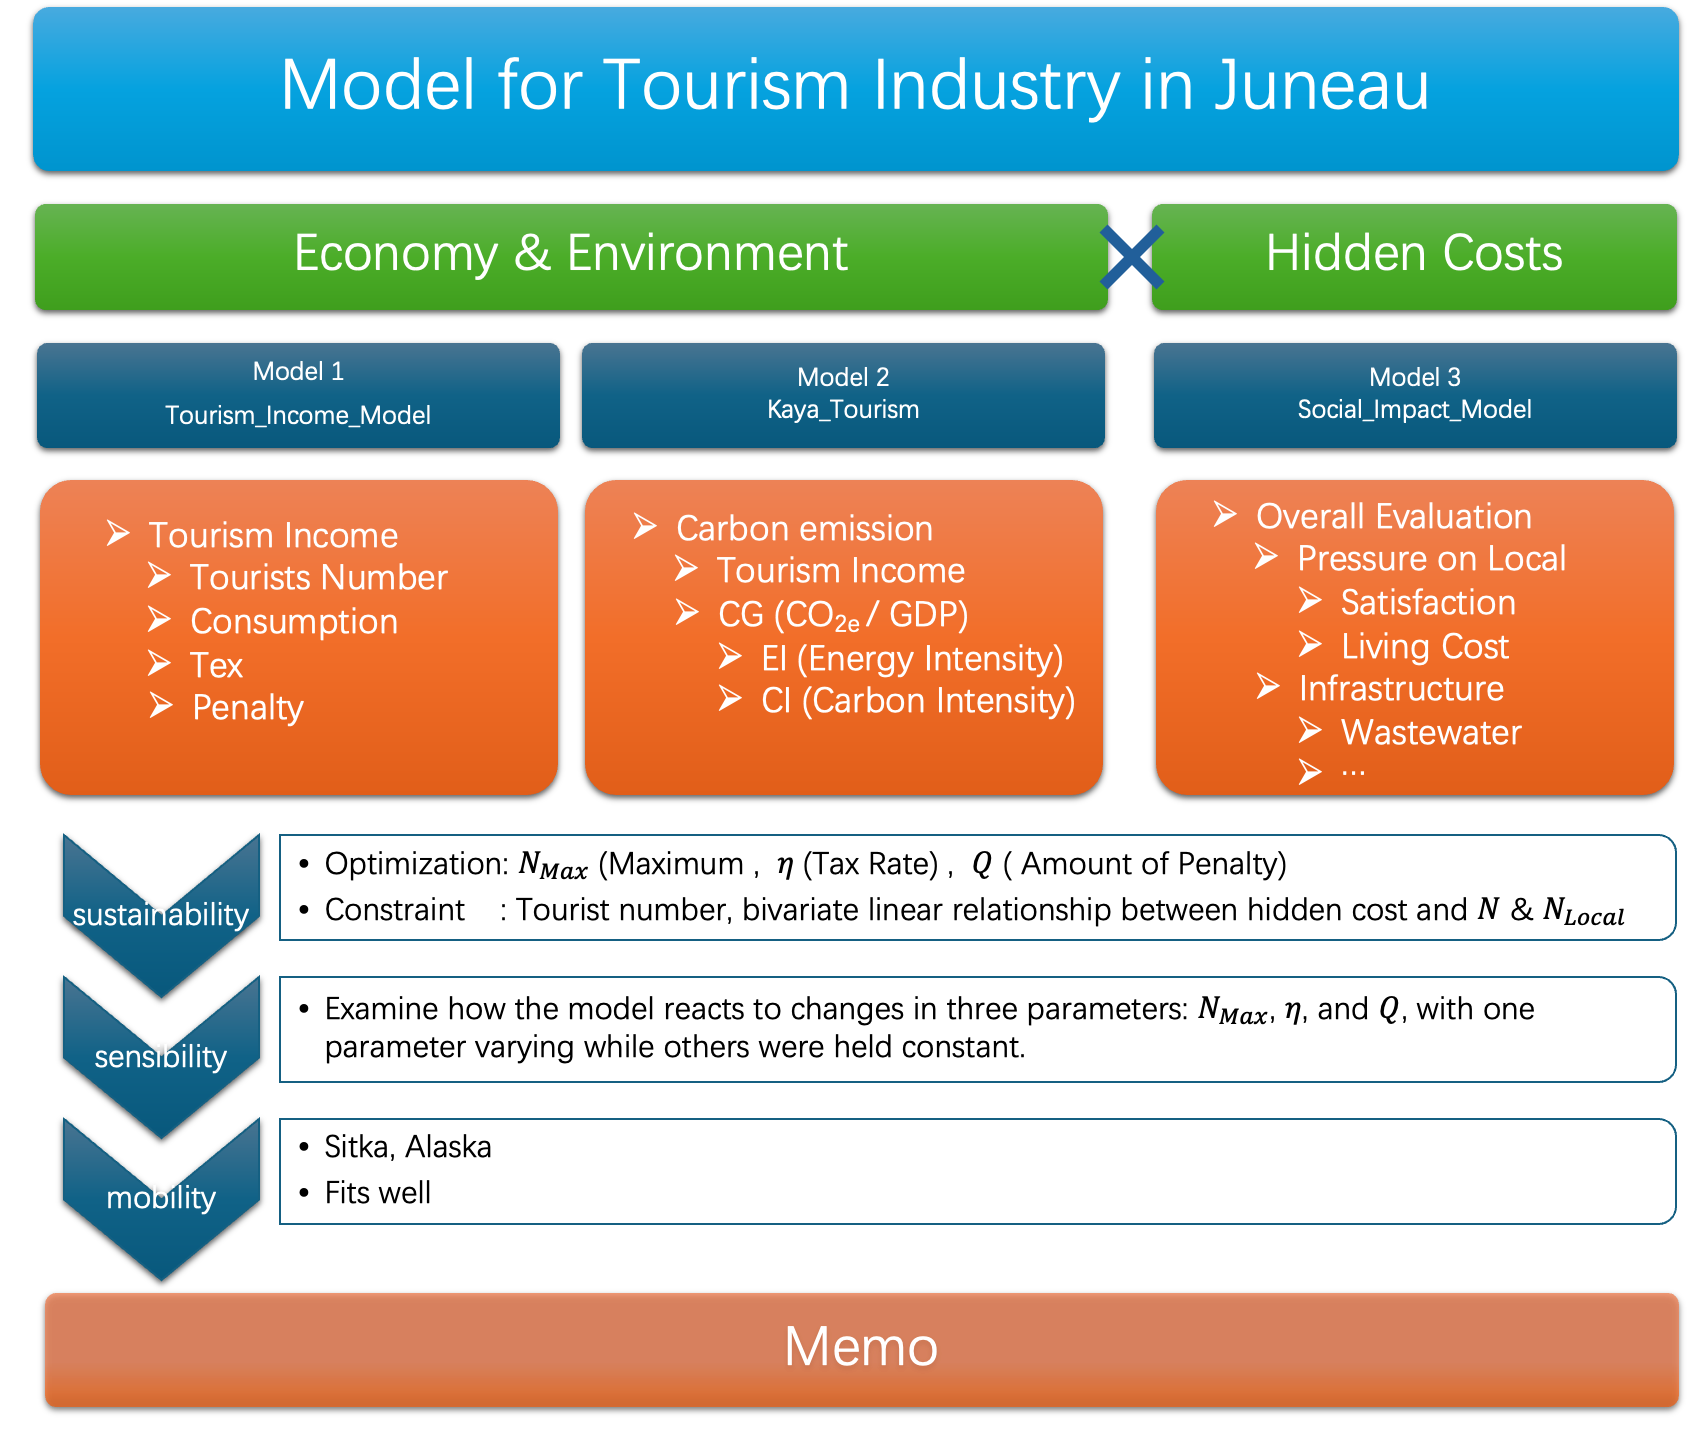
\includegraphics[width=1\textwidth]{FrameWork.jpg} % 插入图片
%     \caption{Our Work Overview Schematic Diagram}
% \end{figure}

